\documentclass{article}

\usepackage{fancyhdr}
\usepackage{extramarks}
\usepackage{amsmath}
\usepackage{amsthm}
\usepackage{amsfonts}
\usepackage{tikz}
\usepackage[plain]{algorithm}
\usepackage{algpseudocode}
\usepackage{listings}
\usepackage{minted}
\usepackage[utf8]{inputenc}
\usepackage[english]{babel}
\usetikzlibrary{automata,positioning}
\usepackage{graphicx}
%
% Basic Document Settings
%


\topmargin=-0.45in
\evensidemargin=0in
\oddsidemargin=0in
\textwidth=6.5in
\textheight=9.0in
\headsep=0.25in

\linespread{1.1}

\pagestyle{fancy}
\lhead{\hmwkClass\ (\hmwkClassInstructor): \hmwkTitle}
\chead{\hspace{4.8in}\hmwkAuthorName}
\rhead{\firstxmark}
\lfoot{\lastxmark}
\cfoot{\thepage}

\renewcommand\headrulewidth{0.4pt}
\renewcommand\footrulewidth{0.4pt}

\setlength\parindent{0pt}

%
% Create Problem Sections
%

\newcommand{\enterProblemHeader}[1]{
    \nobreak\extramarks{}{Problem \arabic{#1} continued on next page\ldots}\nobreak{}
    \nobreak\extramarks{Problem \arabic{#1} (continued)}{Problem \arabic{#1} continued on next page\ldots}\nobreak{}
}

\newcommand{\exitProblemHeader}[1]{
    \nobreak\extramarks{Problem \arabic{#1} (continued)}{Problem \arabic{#1} continued on next page\ldots}\nobreak{}
    \stepcounter{#1}
    \nobreak\extramarks{Problem \arabic{#1}}{}\nobreak{}
}

\setcounter{secnumdepth}{0}
\newcounter{partCounter}


%
% Homework Problem Environment
%
% This environment takes an optional argument. When given, it will adjust the
% problem counter. This is useful for when the problems given for your
% assignment aren't sequential. See the last 3 problems of this template for an
% example.
%


%
% Homework Details
%   - Title
%   - Due date
%   - Class
%   - Section/Time
%   - Instructor
%   - Author
%

\newcommand{\hmwkTitle}{Homework 1}
\newcommand{\hmwkDueDate}{Friday, Feb 5, 2016}
\newcommand{\hmwkClass}{DS-GA 1003}
\newcommand{\hmwkClassInstructor}{Professor David Ronsenberg}
\newcommand{\hmwkAuthorName}{Yuhao Zhao}
\newcommand{\hmwknetid}{Yz3085}
\newcommand{\hmwksubtitle}{Ridge Regression and SGD}

%
% Title Page
%

\title{
    \vspace{2in}
    \textmd{\textbf{\hmwkClass:\ \hmwkTitle \\ \hmwksubtitle }}\\
    \vspace{1in}
    \normalsize\vspace{0.1in}\small{Due\ on\ \hmwkDueDate}\\
    \vspace{0.1in}\large{\textit{\hmwkClassInstructor}}
    \vspace{3in}
}

\author{\textbf{\hmwkAuthorName} \\ \textbf{\hmwknetid }}
\date{}

\renewcommand{\part}[1]{\textbf{\large Part \Alph{partCounter}}\stepcounter{partCounter}\\}

%
% Various Helper Commands
%

% Useful for algorithms
\newcommand{\alg}[1]{\textsc{\bfseries \footnotesize #1}}

% For derivatives
\newcommand{\deriv}[1]{\frac{\mathrm{d}}{\mathrm{d}x} (#1)}

% For partial derivatives
\newcommand{\pderiv}[2]{\frac{\partial}{\partial #1} (#2)}

% Integral dx
\newcommand{\dx}{\mathrm{d}x}

% Alias for the Solution section header
\newcommand{\solution}{\textbf{\large Solution}}

% Probability commands: Expectation, Variance, Covariance, Bias
\newcommand{\E}{\mathrm{E}}
\newcommand{\Var}{\mathrm{Var}}
\newcommand{\Cov}{\mathrm{Cov}}
\newcommand{\Bias}{\mathrm{Bias}}


\newenvironment{problem}[2][$\bullet$]{\begin{trivlist}\large
		\item[\hskip \labelsep {\bfseries #1}\hskip \labelsep {\bfseries #2.}]}  {\end{trivlist}}

\newenvironment{sub}[2][$-$]{\begin{trivlist}
		\item[\hskip \labelsep {\bfseries #1}\hskip \labelsep {\bfseries #2.}]}  {\end{trivlist}}
\newenvironment{lemma}[2][Lemma]{\begin{trivlist}
		\item[\hskip \labelsep {\bfseries #1}\hskip \labelsep {\bfseries #2.}]}{\end{trivlist}}
\newenvironment{exercise}[2][Exercise]{\begin{trivlist}
		\item[\hskip \labelsep {\bfseries #1}\hskip \labelsep {\bfseries #2.}]}{\end{trivlist}}

\newenvironment{question}[2][Question]{\begin{trivlist}
		\item[\hskip \labelsep {\bfseries #1}\hskip \labelsep {\bfseries #2.}]}{\end{trivlist}}
\newenvironment{corollary}[2][Corollary]{\begin{trivlist}
		\item[\hskip \labelsep {\bfseries #1}\hskip \labelsep {\bfseries #2.}]}{\end{trivlist}}

\begin{document}

\maketitle

\pagebreak


%\lstinputlisting{hw1_skeleton_code.py}

\section{2. Linear Regression }
\begin{problem}{\large{2.1 Feature Normalization}}
\end{problem}

\begin{minted}{python}
def feature_normalization(train, test):
	"""Rescale the data so that each feature in the training set is in
	the interval [0,1], and apply the same transformations to the test
	set, using the statistics computed on the training set.
	
	Args:
	train - training set, a 2D numpy array of size (num_instances, num_features)
	test  - test set, a 2D numpy array of size (num_instances, num_features)
	Returns:
	train_normalized - training set after normalization
	test_normalized  - test set after normalization
	
	"""
	shape = train.shape
	b = np.min(train,axis = 0)
	a = np.max(train,axis = 0) - b
	
	return ((train - b)/ a , (test - b)/a)
\end{minted}


\begin{problem}{2.2 Gradient Descent Setup}
\end{problem}

In this problem I will assume each individual input is an column vector, thus the gradient, and $\theta$ are column vectors as well


\begin{sub}{2.2.1}
\end{sub}

For each individual $x \in R^d, h_{\theta} = \theta^T x$. Let $X \in R^{m\times (d +1)}$ be the design matrix of the input data, and $y = (y_1, ... ,y_m)^T$ be the response vector. Then $h_X(\theta) = X \theta$. \\The objective function: 
 $$J(\theta) = \frac{1}{2m} ||X \theta - y||_{L2}^2$$

\begin{sub}{2.2.2}
\end{sub}

The gradient of $J $  is :\\ 
$$ \nabla_{\theta} J(\theta) = \frac{1}{m} X^T(X\theta - y)$$

\begin{sub}{2.2.3}
\end{sub}

By Taylor expansion of $J(\theta)$ at $\theta$, we have  the first order approximation for J is :\\ $$J(\theta+\eta\Delta) - J(\theta) =  (\theta+\eta\Delta - \theta)^T  \nabla J(\theta)   =  \frac{1}{m} \eta \Delta^T X^T(X\theta - y) $$


\begin{sub}{2.2.4}
\end{sub}

The $\theta$ updating rule for gradient descent is:\\
$$ \theta_{i+1} = \theta_{i} - \frac{\eta}{m} X^T(X\theta_{i} - y) $$

\pagebreak

\begin{sub}{2.2.5}
	
\end{sub}

\begin{minted}{python}
def compute_square_loss(X, y, theta):
	"""
	Given a set of X, y, theta, compute the square loss for predicting y with X*theta
	
	Args:
	X - the feature vector, 2D numpy array of size (num_instances, num_features)
	y - the label vector, 1D numpy array of size (num_instances)
	theta - the parameter vector, 1D array of size (num_features)
	
	Returns:
	loss - the square loss, scalar
	"""
	loss = 0 #initialize the square_loss
	m = X.shape[0] *1.0
	theta = np.array([theta]).T
	y = np.array([y]).T
	
	return (1/(2*m) *  np.linalg.norm(np.dot(X,theta) - y)**2)

\end{minted}

\begin{sub}{2.2.6}
\end{sub}

For data $X = \begin{bmatrix}
1 &2&3&4\\ 4&3&2&1
\end{bmatrix}$, y= $\begin{bmatrix} 0\\1 \end{bmatrix} $ and $\theta = \begin{bmatrix} 1\\0\\1\\0 \end{bmatrix}$. \\The square loss should be $\frac{1}{4} ((4-0)^2 + (6-1)^2) = \frac{41}{4} = 10.25$\\

and the function returns:
\begin{minted}{python}
>>> x = np.array([[1, 2, 3, 4],[4, 3, 2, 1]])
>>> y= np.array([0,1])
>>> theta = np.array([1,0,1,0])
>>> compute_square_loss(x,y,theta)
>>> 10.25
\end{minted}


\begin{sub}{2.2.7}
\end{sub}

\begin{minted}{python}
def compute_square_loss_gradient(X, y, theta):
	"""
	Compute gradient of the square loss (as defined in compute_square_loss), 
	at the point theta.
	
	Args:
	X - the feature vector, 2D numpy array of size (num_instances, num_features)
	y - the label vector, 1D numpy array of size (num_instances)
	theta - the parameter vector, 1D numpy array of size (num_features)
	
	Returns:
	grad - gradient vector, 1D numpy array of size (num_features)
	"""
	m = X.shape[0] *1.0
	theta = np.array([theta]).T
	y = np.array([y]).T
	
	return (1/m * np.dot(X.T,(np.dot(X,theta) - y)) )[:,0]

\end{minted}

\begin{sub}{2.2.8}
\end{sub}

The gradient should be: \\
$\frac{1}{2} \times \begin{bmatrix}
 1&4\\ 2&3 \\ 3&2 \\4&1
\end{bmatrix}
\begin{bmatrix}
4\\5
\end{bmatrix} = \frac{1}{2}\begin{bmatrix}
24\\23\\22\\21
\end{bmatrix} = \frac{1}{2}\begin{bmatrix}
12\\11.5\\11\\10.5
\end{bmatrix}$ 

and the function returns:
\begin{minted}{python}
>>> compute_square_loss_gradient(x,y,theta)
>>> array([ 12. ,  11.5,  11. ,  10.5])
\end{minted}


\begin{problem}{2.3 Gradient Checker}
\end{problem}

\begin{sub}{2.3.1}
\end{sub}

\begin{minted}{python}
def grad_checker(X, y, theta, epsilon=0.01, tolerance=1e-4): 
	"""Implement Gradient Checker
	Check that the function compute_square_loss_gradient returns the
	correct gradient for the given X, y, and theta.
	
	Args:
	X - the feature vector, 2D numpy array of size (num_instances, num_features)
	y - the label vector, 1D numpy array of size (num_instances)
	theta - the parameter vector, 1D numpy array of size (num_features)
	epsilon - the epsilon used in approximation
	tolerance - the tolerance error
	
	Return:
	A boolean value indicate whether the gradient is correct or not
	
	"""
	true_gradient = compute_square_loss_gradient(X, y, theta) #the true gradient
	num_features = theta.shape[0]
	approx_grad = np.zeros(num_features) #Initialize the gradient we approximate
	
	y = np.array([y]).T
	approx_matrix = np.identity(num_features) #initialize the directional derivatives
	approx_grad = np.apply_along_axis(lambda t:(compute_square_loss(X,y,theta+ epsilon*t) 
	- compute_square_loss(X,y,theta- epsilon*t))/(2*epsilon) ,0,approx_matrix) 
	#apply the gradient function to directional derivatives 
	
	checker = np.linalg.norm(true_gradient - approx_grad)
	
	return checker < tolerance

\end{minted}

\begin{sub}{2.3.2}
\end{sub}
\begin{minted}{python}
def generic_gradient_checker(X, y, theta, objective_func,
gradient_func, epsilon=0.01, tolerance=1e-4):
	"""
	The functions takes objective_func and gradient_func as parameters.
	And check whether gradient_func(X, y, theta) returned
	the true gradient for objective_func(X, y, theta).
	Eg: In LSR, the objective_func = compute_square_loss,
	and gradient_func = compute_square_loss_gradient
	"""
	true_gradient = gradient_func(X, y, theta) #the true gradient
	num_features = theta.shape[0]
	approx_grad = np.zeros(num_features) #Initialize the gradient we approximate
	
	y = np.array([y]).T
	approx_matrix = np.identity(num_features)
	approx_grad = np.apply_along_axis(lambda t: (objective_func(X,y,theta+ epsilon*t)
	- objective_func(X,y,theta- epsilon*t))/(2*epsilon) ,0,approx_matrix)
	
	checker = np.linalg.norm(true_gradient - approx_grad)
	return checker < tolerance

\end{minted}


\begin{problem}{2.4 Batch Gradient Descent}
\end{problem}

\begin{sub}{2.4.1}
\end{sub}

\begin{minted}{python}
def batch_grad_descent(X, y, alpha=0.1, num_iter=1000, check_gradient=False):
	"""
	In this question you will implement batch gradient descent to
	minimize the square loss objective
	
	Args:
	X - the feature vector, 2D numpy array of size (num_instances, num_features)
	y - the label vector, 1D numpy array of size (num_instances)
	alpha - step size in gradient descent
	num_iter - number of iterations to run 
	check_gradient - a boolean value indicating whether checking the 
	gradient when updating
	
	Returns:
	theta_hist - store the the history of parameter vector in iteration,
	2D numpy array of size (num_iter+1, num_features) 
	for instance, theta in iteration 0 should be theta_hist[0],
	 theta in ieration (num_iter) is theta_hist[-1]
	loss_hist - the history of objective function vector, 
	1D numpy array of size (num_iter+1) 
	"""
    num_instances, num_features = X.shape[0], X.shape[1]
    theta_hist = np.zeros((num_iter+1, num_features))  #Initialize theta_hist
    loss_hist = np.zeros(num_iter+1) #initialize loss_hist
    theta = np.ones(num_features) #initialize theta
    
    theta_hist[0,:] = theta
    loss_hist[0] = compute_square_loss(X,y,theta)
    
    if not check_gradient:
	    for i in list(xrange(1,num_iter+1)):
		    theta = theta - compute_square_loss_gradient(X,y,theta)*alpha
		    theta_hist[i,:] = theta 
		    loss_hist[i] = compute_square_loss(X,y,theta)
    else:
	    for i in list(xrange(1,num_iter+1)): 
		    if grad_checker(X,y,theta,epsilon=0.01, tolerance=1e-4):
			    theta = theta - compute_square_loss_gradient(X,y,theta)*alpha
			    theta_hist[i,:] = theta 
			    loss_hist[i] = compute_square_loss(X,y,theta)        
		    else:
			    print('error, please check gradient function')
			    return 
    return (theta_hist,loss_hist)

\end{minted}

\begin{sub}{2.4.2}
\end{sub}

\begin{minted}{python}
def step_checker(X, y, alpha = [0.1], num_iter=1000):
	"""
	Comput the square loss objective function for given alpha values
	
	Args:
	X - the feature vector, 2D numpy array of size (num_instances, num_features)
	y - the label vector, 1D numpy array of size (num_instances)
	alpha - step size in gradient descent
	num_iter - number of iterations to run 
	
	Returns:
	loss_hist - the history of objective function vector, 
	2D numpy array of size (len(alpha) ,num_iter+1) 
	"""
	num_alpha = len(alpha)
	loss_hist  = np.zeros((num_alpha, 1001))
	for i in list(xrange(num_alpha)):
	loss_hist[i,:] = batch_grad_descent(X,y,alpha[i],num_iter=1000)[1]
	
	return loss_hist
\end{minted}

\begin{minted}{python}
    alpha = [0.5,0.1,0.05,0.01] 
    temp = step_checker(X_train,y_train,alpha,1000)
    plt.ylabel('objective function')
    plt.xlabel('step')
    for i in list(xrange(len(alpha))):
	    plt.plot(temp[i,:],label = 'step size = '+ str(alpha[i]) + 
		    ('(Diverge)' if np.isnan(temp[i,-1]) else '(Converge)' ))   
    plt.legend()
    plt.show()
\end{minted}
\begin{center}
	 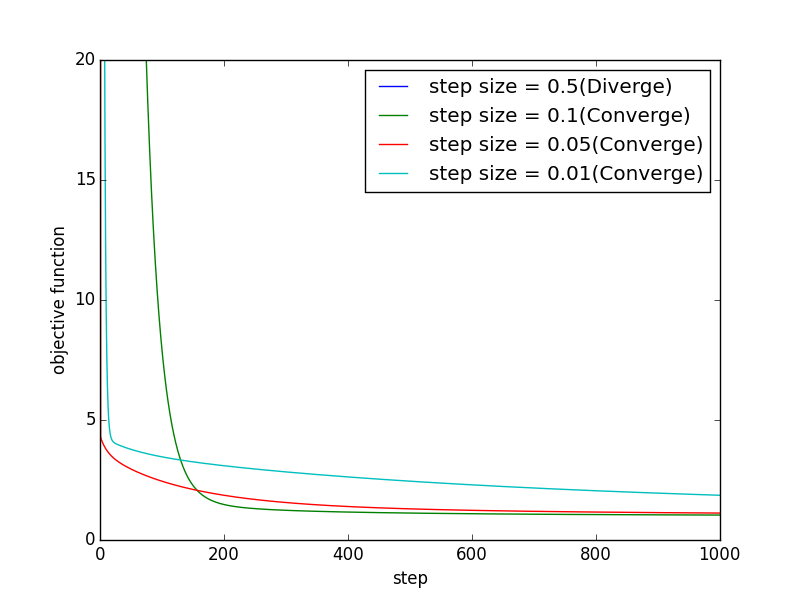
\includegraphics[height = 4in]{2_4_2.png}
\end{center}

From the above figure, we can see that the objective function diverges when step size is large(0.5). And it converges most quickly when step size is 0.05. What's more, minimization with different step size does not converge to the same values. 

\begin{sub}{2.4.3}
\end{sub}

\begin{minted}{python}
def batch_line_search_grad_descent(X,y,num_iter=1000,tau = 0.5,c = 0.5,alpha_0 = 0.5):

	"""
	use backtracking line search to minimize the square loss objective
	
	Args:
	X - the feature vector, 2D numpy array of size (num_instances, num_features)
	y - the label vector, 1D numpy array of size (num_instances)
	num_iter - number of iterations to run 
	tau,c,alpha_0 - float number, the parameters used for step search 
	
	Returns:
	theta_hist - store the the history of parameter vector in iteration
	loss_hist - the history of objective function vector 
	time_list - the time used to each the step size for each iteration, 1D numpy array
	"""

	num_instances, num_features = X.shape[0], X.shape[1]
	theta_hist = np.zeros((num_iter+1, num_features))  #Initialize theta_hist
	loss_hist = np.zeros(num_iter+1) #initialize loss_hist
	theta = np.ones(num_features) #initialize theta
	
	theta_hist[0,:] = theta
	loss_hist[0] = compute_square_loss(X,y,theta)
	time_list = np.zeros(num_iter)
	
	for i in list(xrange(1,num_iter+1)):
		alpha = alpha_0 
		p = -compute_square_loss_gradient(X,y,theta)
		t = 1.0 *c * np.linalg.norm(p)**2
		temp1 = compute_square_loss(X,y,theta)  #find current loss
		current  =time.time()
		while 1: 
			temp2 = compute_square_loss(X,y,theta+ alpha *p) 
			#compute loss at current step
			if   temp2 >  temp1 - alpha * t: 
				alpha = tau* alpha  #shrink alpha
				continue
			else:
				time_list[i-1] = time.time() -current
				break
	
		theta = theta+ alpha *p
		theta_hist[i,:] = theta 
		loss_hist[i] = temp2
		
	return (theta_hist,loss_hist,time_list)  	 
	
current1  = datetime.datetime.now()
batch_line_search_grad_descent(X_train,y_train)
print('runing time of backtracking line search GD:' + str(datetime.datetime.now() -current1) )

current2  = datetime.datetime.now()
batch_grad_descent(X_train,y_train)
print('runing time of Batch GD :' + str(datetime.datetime.now() -current2) )

current3 = np.mean(batch_line_search_grad_descent(X_train,y_train)[2])
print('average extra runing time for step search: ' + str(current3) )

current4  = time.time()
compute_square_loss_gradient(X_train,y_train,theta)
print('runing time for computing gradient ' + str(time.time() - current4) )


>>>runing time of backtracking line search: GD0:00:00.121715
>>>runing time of Batch GD: 0:00:00.038145
>>>average extra runing time for step search: 4.21249866486e-05
>>>runing time for computing gradient 6.48498535156e-05

\end{minted}



The output by implementing this method is as following: 
\begin{center}
	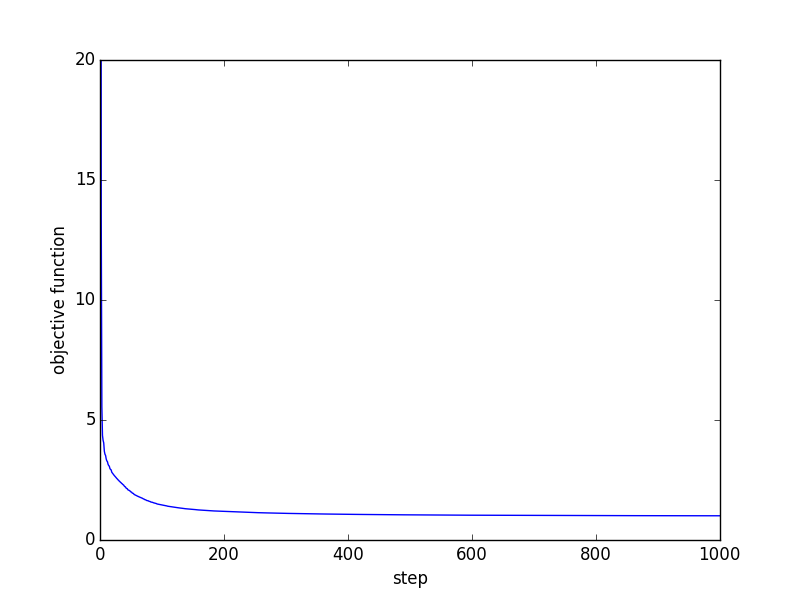
\includegraphics[height = 3.6in]{2_4_3.png}
\end{center}

From the graph we can see that the backtracking line search GD method converges almost the same faster as the best regular batch GD. However the running time for bath GD is shorter than the  backtracking line search GD. The extra time to run backtracking line search is shorter than it takes to compute the gradient. 

\begin{problem}{Ridge Regression}
\end{problem}

\begin{sub}{2.5.1}
\end{sub} 

Since $J(\theta)  = \frac{1}{2m} \sum_{i=1}^{m} (h_{\theta}(x_i) - y_i)^2 + \lambda \theta^T \theta=  \frac{1}{2m} ||X \theta||_{L2}^2 + \lambda ||\theta||_{L2}^2$\\
Then the gradient is:
$$\nabla_{\theta} J(\theta) = \frac{1}{m} X^T(X\theta - y) + 2\lambda \theta$$

The expression for updating $\theta$ is:
$$\theta_{i} = \theta_{i - 1 } -\eta[ \frac{1}{m} X^T(X\theta_{i-1} - y) + 2\lambda \theta_{i-1}]$$

\begin{sub}{2.5.2}
\end{sub}

\begin{minted}{python}
def compute_regularized_square_loss_gradient(X, y, theta, lambda_reg):
	"""
	Compute the gradient of L2-regularized square loss function given X, y and theta
	
	Args:
	X - the feature vector, 2D numpy array of size (num_instances, num_features)
	y - the label vector, 1D numpy array of size (num_instances)
	theta - the parameter vector, 1D numpy array of size (num_features)
	lambda_reg - the regularization coefficient
	
	Returns:
	grad - gradient vector, 1D numpy array of size (num_features)
	"""
	return compute_square_loss_gradient(X,y,theta) + 2*lambda_reg*theta 
\end{minted}

\begin{sub}{2.5.3}
\end{sub}

\begin{minted}{python}
def regularized_grad_descent(X, y, alpha=0.1, lambda_reg=1, num_iter=1000):
	"""
	Args:
	X - the feature vector, 2D numpy array of size (num_instances, num_features)
	y - the label vector, 1D numpy array of size (num_instances)
	alpha - step size in gradient descent
	lambda_reg - the regularization coefficient
	numIter - number of iterations to run 
	
	Returns:
	theta_hist - the history of parameter vector, 2D numpy array of size
				 (num_iter+1, num_features) 
	loss_hist - the history of regularized loss value, 1D numpy array
	"""
	(num_instances, num_features) = X.shape
	theta = np.ones(num_features) #Initialize theta
	theta_hist = np.zeros((num_iter+1, num_features))  #Initialize theta_hist
	loss_hist = np.zeros(num_iter+1) #Initialize loss_hist
	
	theta_hist[0,:] = theta
	loss_hist[0] = compute_square_loss(X,y,theta) + lambda_reg*np.linalg.norm(theta)**2
	
	for i in list(xrange(1,num_iter+1)):
		theta = theta - compute_regularized_square_loss_gradient(X,
					y,theta,lambda_reg)*alpha
		theta_hist[i,:] = theta 
		loss_hist[i] = compute_square_loss(X,y,theta)
						+ lambda_reg*np.linalg.norm(theta)**2	
	return (theta_hist,loss_hist)    
\end{minted}

\pagebreak

\begin{sub}{2.5.4}
\end{sub}
\begin{center}
	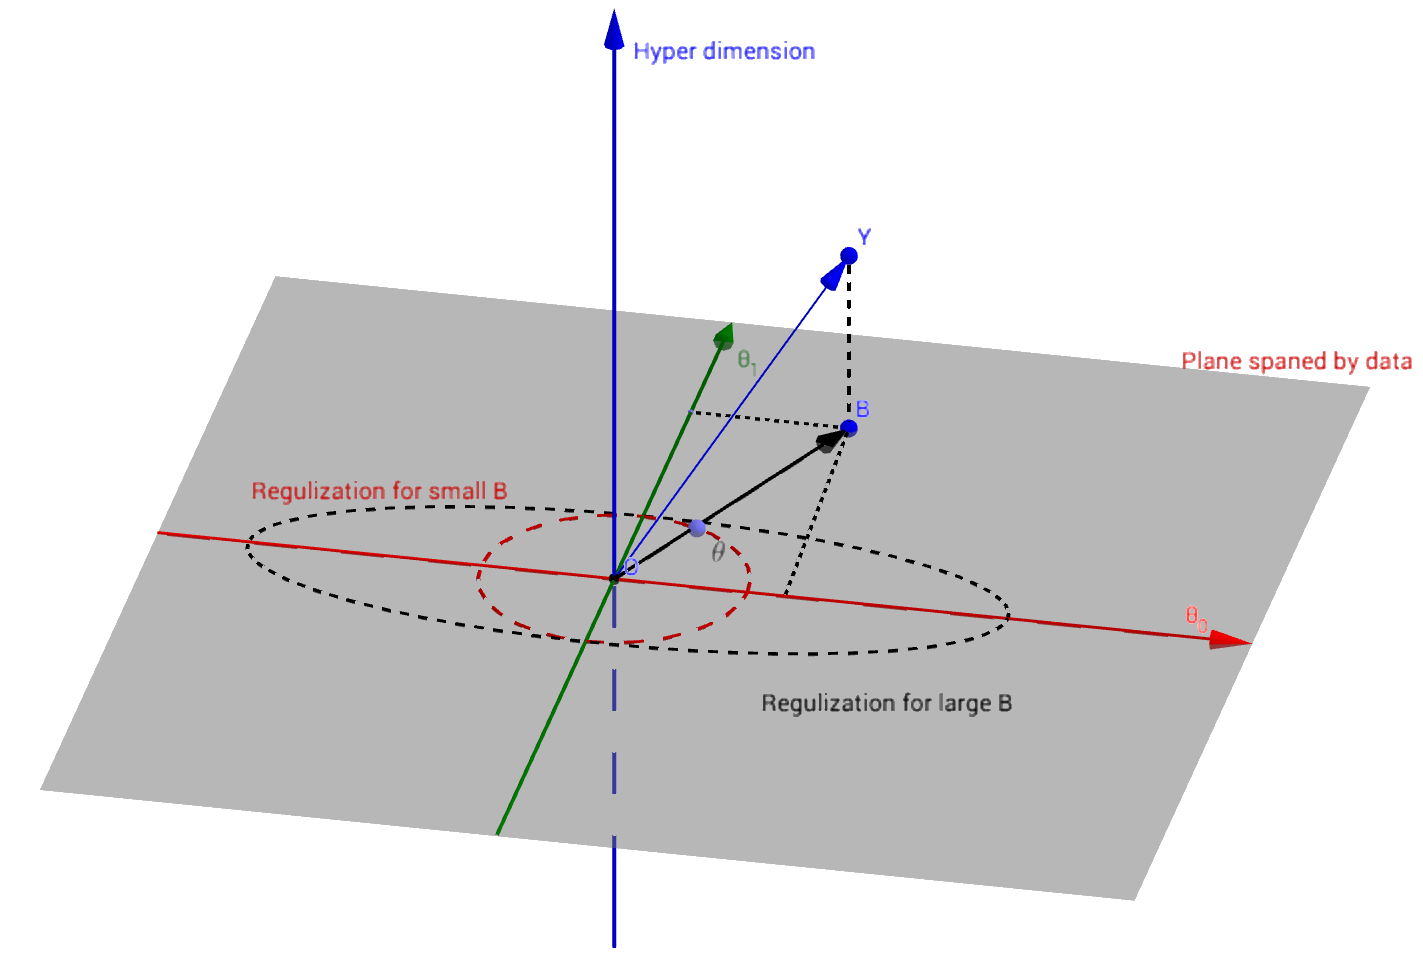
\includegraphics[height = 3in]{2_5_3.png}
\end{center}

The geometrical interpretation of the square loss solution, in an N-dimensional space is the projection of data vector y onto the subspace spanned by the data (basis functions). The solution is the corresponding coordinates in the space. If we visualize the N-d space onto 3D, which x-axis represents the bias $\theta_0$, y-axis represents another N-1 D parameters and z-axis represents other hyper-dimensions, the L2 regularization regularized the solution inside the unit circle. If we initialize a very large B for the bias term for all the data, it's equivalent to magnify the basis for $\theta_0$ by B. In other words, it a transformation of the regularization. After the transformation, the regularization becomes a ellipsoid.As we can see from the graph above, when we project the coefficients into the regularization region,  the new regularization on bias term will become less effective. We can make the regularization as weak as we want by initializing a large enough B. 

\begin{sub}{2.5.5}
\end{sub}
\begin{minted}{python}
	def Ridge_lambda_search(X_train , y_train,X_test= , y_test ,
	 lambda_=[10**-7,10**-5,10**-3,10**-1,1,10,100]): 
	"""
	checking the convergency for different regulization lambda
	returns the last element of loss_hist returned by regularized_grad_descent
	"""
	
	res_training =  np.zeros(len(lambda_))
	res_testing = np.zeros(len(lambda_))
	
	for i in list(xrange(len(lambda_))):
		temp = regularized_grad_descent(X_train,y_train,lambda_reg=lambda_[i])
		theta = temp[0][-1,:]
		res_testing[i] = compute_square_loss(X_test,y_test,theta)
		res_training[i] = compute_square_loss(X_train,y_train,theta)
	
	return (res_testing,res_training)

>>> Ridge_lambda_search(X_train,t_train,X_test,y_test)[0]
>>> array([  1.45465079e+000, 1.45406016e+000, 1.40092244e+000
	, 3.40518038e+001, 2.93230478e+145, nan, nan])
	
plt.close('all')
try_list = np.linspace(10**-7,10**-1,100)
t_2_5 = Ridge_lambda_search(X_train, y_train, X_test, y_test, lambda_=try_list)
fig = plt.figure()
ax = fig.add_subplot(111)
ax.set_ylim([0,3])
ax.set_xlabel('$log_{10}(\lambda)$')
ax.set_ylabel('loss')

plt.plot(np.log10(try_list),t_2_5[0],label = 'validation lost')
plt.plot(np.log10(try_list),t_2_5[1],label = 'training lost')
plt.legend()
plt.show()

lambda_opt=  try_list[np.where(t_2_5[0] ==np.min(t_2_5[0]))[0][0]]

\end{minted}
\begin{center}
	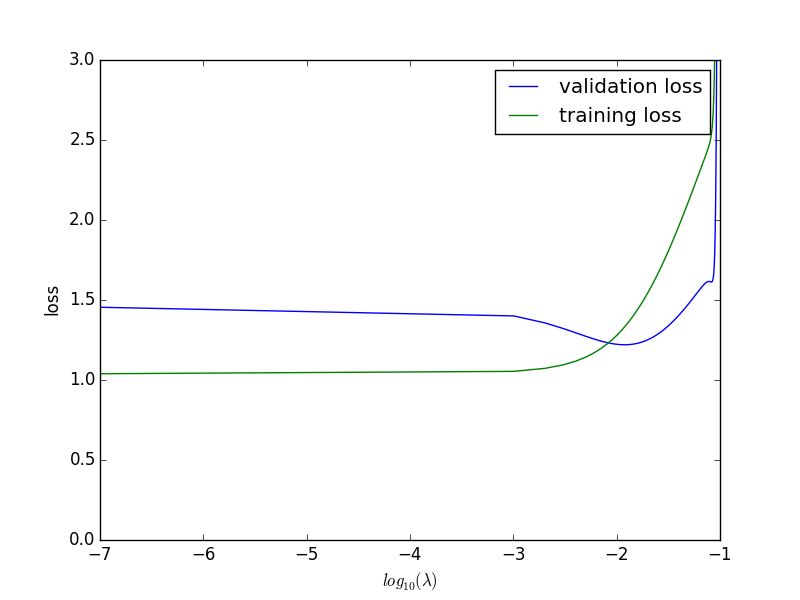
\includegraphics[height = 3in]{2_5_5.png}
\end{center}

After searching the $\lambda$ widely from $\{ 10^{-7},10^{-5},10^{-3},10^{-1},1,10,100 \}$, the algorithm converges  from $\lambda = 10^{-7}$ to $10^{-1}$. From the graph, we can see that the validation loss minimizes at around $log_{10}(\lambda) = -2$. Indeed, the optimal $\lambda$ is 0.0121213.

\begin{sub}{2.5.6}
\end{sub}

\begin{minted}{python}
df = pd.read_csv('hw1-data.csv', delimiter=',')
X = df.values[:,:-1]
y = df.values[:,-1]
X_train, X_test, y_train, y_test = train_test_split(X, y, test_size =100, random_state=10)
X_train, X_test = feature_normalization(X_train, X_test)

try_list = np.linspace(0,10,110)
res = np.ones(110)

for i,B in enumerate(try_list):
	data = (np.hstack((X_train, B*np.ones((X_train.shape[0], 1)))),
	np.hstack((X_test, B*np.ones((X_test.shape[0], 1)))))

res[i] = Ridge_lambda_search(data[0],y_train,data[1],y_test,lambda_ = [lambda_opt])[1][0]

\end{minted}

\begin{center}
	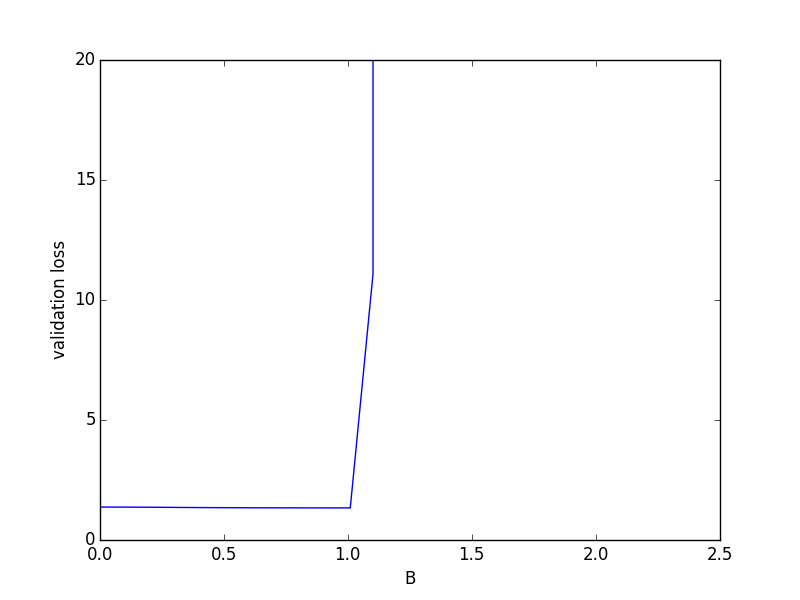
\includegraphics[height = 3in]{2_5_6.png}
\end{center}

According to the plot, we can see that the validation loss actually explode for initial B greater than 1. Therefore, regularizing the bias help to reduce the loss in this data. 

\begin{sub}{2.5.7}
\end{sub}

\begin{minted}{python}
>>>current = time.time()
...compute_regularized_square_loss_gradient(X_train,
y_train,theta = np.ones(49),lambda_reg = lambda_opt)
...print (time.time() - current)
>>>3.02069187164e-05
\end{minted}

The average time it takes for a single gradient step is 3.02069187164e-05 second

\begin{sub}{2.5.8}
\end{sub}

Since our target is to minimize the validation loss, in deployment, we should choose the $\theta$ corresponding to the minimum square loss.





\begin{problem}{2.6 Stochastic Gradient Decent}
\end{problem}

\begin{sub}{2.6.1}
\end{sub}

For SGD algorithm, we randomly select one data instance and compute the gradient according to this single vector. Therefore the update rule for $\theta$ is :\\
$$\theta_{i} = \theta_{i-1} - \eta x_{i-1} (\theta_{i-1}^Tx_{i-1}-y_{i-1} ) $$

\begin{sub}{2.6.2}
\end{sub}

\begin{minted}{python}
def stochastic_grad_descent(X, y, alpha=0.1, lambda_reg=1, num_iter=1000):
"""
In this question you will implement stochastic gradient descent with a regularization term

Args:
X - the feature vector, 2D numpy array of size (num_instances, num_features)
y - the label vector, 1D numpy array of size (num_instances)
alpha - string or float. step size in gradient descent

if alpha is a float, then the step size in every iteration is alpha.
if alpha == "1/sqrt(t)", alpha = 1/sqrt(t)
if alpha == "1/t", alpha = 1/t
lambda_reg - the regularization coefficient
num_iter - number of epochs (i.e number of times) to go through the whole training set

Returns:
theta_hist - the history of parameter vector, 
3D numpy array of size (num_iter, num_instances, num_features) 
loss hist - the history of regularized loss function vector, 
2D numpy array of size(num_iter, num_instances)
"""
num_instances, num_features = X.shape[0], X.shape[1]
theta = np.ones(num_features) #Initialize theta

theta_hist = np.zeros((num_iter, num_instances, num_features))  #Initialize theta_hist
loss_hist = np.zeros((num_iter, num_instances)) #Initialize loss_hist
t = 0

for n in list(xrange(num_iter)):
generator = np.random.permutation(list(xrange(num_instances))) # define ramdom sampling sequence

for i in list(xrange(0,num_instances)):
	t+=1.0
	num = generator[i]
	if alpha == "1/sqrt(t)":
		theta = theta - 1/np.sqrt(t) *( (np.inner(X[num,:], theta)-y[num]) 
			*X[num,:] + 2*lambda_reg*theta)
	elif alpha  == "1/t":
		theta = theta - (1/(t)) * ( (np.inner(X[num,:], theta)-y[num]) 
			*X[num,:] + 2*lambda_reg*theta)
	else:
		theta = theta - alpha * ((np.inner(X[num,:], theta)-y[num]) 
			*X[num,:] + 2*lambda_reg*theta)
	
	theta_hist[n][i,:] = theta 
	loss_hist[n,i] = compute_square_loss(X,y,theta)+lambda_reg*np.linalg.norm(theta)**2

return (theta_hist,loss_hist)    

\end{minted}

\begin{sub}{2.6.3}
\end{sub}

\begin{center}
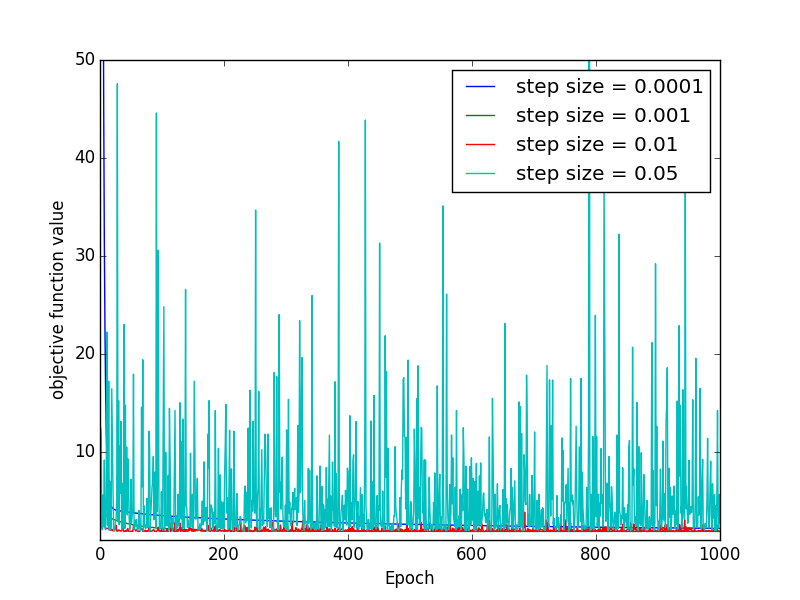
\includegraphics[height = 2.3in]{2_6_3_1.png}
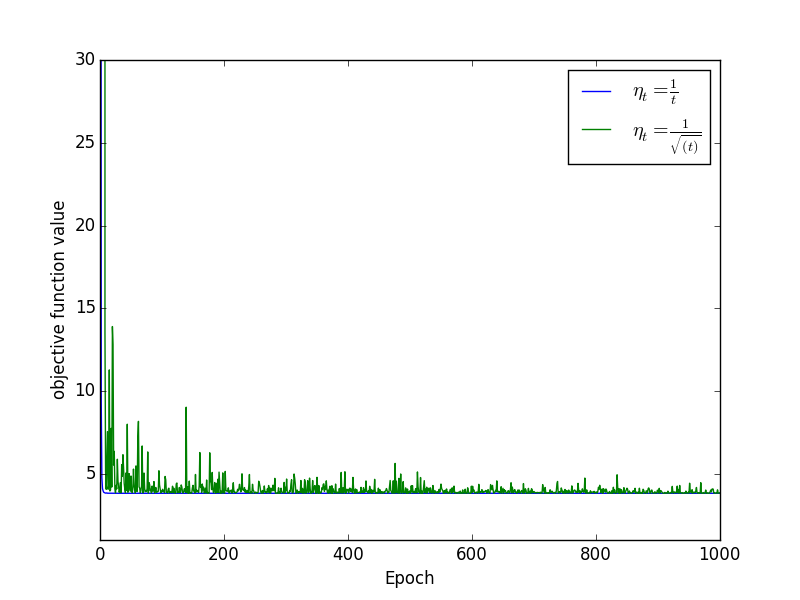
\includegraphics[height = 2.3in]{2_6_3_2.png}
\end{center}

From the two plots above, we can see that the fixed step SGD algorithm does not guarantee convergence. For example, when step size= 0.05, the objective function are oscillating between 0 and 50. For decreasing step size SGD, the $\frac{1}{t}$ rule works better than$\frac{1}{\sqrt{t}}$ , and they both converge. What's more, we notice that the $\frac{1}{t}$ rule converges more quickly than any of the fix step algorithms. In conclusion, if we chose a appropriate step size and regularization term, the SGD converges faster than GD.

\begin{sub}{2.6.4}
	\end{sub}

\begin{center}
	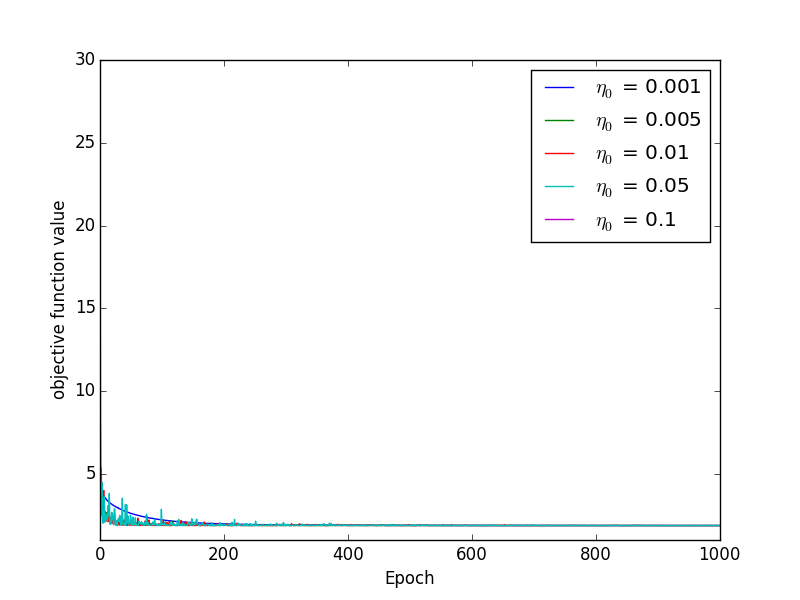
\includegraphics[height = 3in ]{2_6_4.png}
\end{center}

For $\eta_0 \in [0.001, 0.05]$, the SGD with $\frac{\eta_0}{1+\eta_0\lambda t}$ rule converges. However it works no better than $\eta  = \frac{1}{t}$ rule.

\begin{sub}{2.6.5}
\end{sub}

\begin{minted}{python}
>>>current  = time.time()
...stochastic_grad_descent(X_train,y_train,alpha = '1/t')
...print('running time for a single epoch of SGD is ' + str((time.time() -current)/1000) + ' second')
>>>running time for a single epoch of SGD is 0.00253006601334 second
\end{minted}
\pagebreak
\begin{sub}{2.6.6}
\end{sub}
We notice that the running time for a single epoch of SGD is longer than that for GD. Therefore, if our goal is to minimize the total time we should choose GD. Otherwise, if we want to minimize the total numbers of epochs (steps), we should choose SGD.\\

\section{3. Risk Minimization}

\begin{problem}{3.1}
\end{problem}

For the square loss, $l(\hat{y},y) = \frac{1}{2}(y-\hat{y})^2, R(f) = E(l(f(x),y)),R(f^*) = \inf_f R(f)$\\
$$R(f) = \frac{1}{2}E[(f(X) - Y)^2] = \frac{1}{2} E[(f(X) - E(Y|X) +E(Y|X) -Y)^2] $$ 
$$ = \frac{1}{2}E[(f(X) - E(Y|X))^2 + (Y - E(Y|X) )^2 +2 (f(X) - E(Y|X))(Y - E(Y|X) )]$$
Since, $E[ (f(X) - E(Y|X))(Y - E(Y|X) )] = E[Y(f(X) - E(Y|X))] - E(E(Y|X)(f(X) - E(Y|X)))$\\
and $E(Y) = E(E(Y|X)), E[ (f(X) - E(Y|X))(Y - E(Y|X) )] = 0$\\
$$R(f)= \frac{1}{2} E[(f(X) - E(Y|X))^2 + (Y - E(Y|X) )^2] $$ 

We notice that $R(f)$ can be minimized when $f^* = E(Y|X)$

\begin{problem}{3.2}
	\end{problem}

For the absolute loss, $l(\hat{y},y)  = |y - \hat{y}|$\\
Since we can always choose $f(X_i)$ independent with each other $X_i's$, the minimum of the expected $L_1$ loss can be found by minimizing the integrate given by:
$$R(f) = \int_{Y\in \mathcal{Y} } |f(X) - Y| p(Y|X) dY $$
For each value of X. Setting the derivative of $R(f)$ with respect to f to zero gives: 
$$\int_{-\infty}^{f(X)} (f(X) -Y) p(Y|X)dY - \int^{\infty}_{f(X)} (f(X) -Y) p(Y|X)dY   = 0$$\\
And this reduces to: 
$$\int_{-\infty}^{f(X)} p(Y|X)dY =  \int^{\infty}_{f(X)} p(Y|X)dY   $$
Since we know that:
$$\int_{-\infty}^{f(X)} p(Y|X)dY + \int^{\infty}_{f(X)} p(Y|X)dY = 1$$
Then,
$$\int_{-\infty}^{f(X)} p(Y|X)dY =  \int^{\infty}_{f(X)} p(Y|X)dY = \frac{1}{2}$$
which says that $f^*$ must be the conditional median of Y.
\end{document}



